\documentclass[11pt]{article}
\usepackage[margin=1in]{geometry}
\usepackage{amsmath,amssymb}
\usepackage{graphicx}
\usepackage{booktabs}
\usepackage{xcolor}
\usepackage{enumitem}
\usepackage{fancyvrb}
\usepackage[colorlinks=true,linkcolor=blue!50!black,urlcolor=blue!50!black,
            citecolor=blue!50!black]{hyperref}

\definecolor{codebg}{gray}{0.96}
\newcommand{\code}[1]{\texttt{#1}}
\newcommand{\GW}{\ensuremath{\Gamma_W}}
\newcommand{\Gc}{\ensuremath{\Gamma_c}}
\newcommand{\Bstar}{\ensuremath{B_\ast}}
\newcommand{\ii}{\ensuremath{\iota}}

\setlength{\parskip}{0.5em}
\setlength{\parindent}{0pt}

\title{\vspace{-1.5em}\textbf{\GW\ --- the Whitham Energetic-Particle Confinement Proxy}\\[0.3em]
\large A standalone, physicist-oriented reference}
\author{}
\date{Documentation revision: 2026-07-13\\[0.2em]
\small Canonical engine: \code{Gamma\_W\_final.py}, md5 \code{b58272e4}}

\begin{document}
\maketitle
\vspace{-2.5em}

\begin{abstract}
\noindent
\GW\ is a fast, \emph{field-only} proxy for prompt energetic-particle (fusion-alpha)
confinement in stellarators and tokamaks. A trapped alpha's \emph{bounce centre}---its
guiding centre averaged over one bounce---drifts slowly across flux surfaces; \GW\ measures
how far, radially, that drift can carry the trapped population before a chosen time $t_\ast$,
using only the equilibrium magnetic field, with no collisional orbit tracing. It rests on
Whitham / bounce-averaged adiabatic theory: the second adiabatic invariant $J$ is conserved
along the drift, so the bounce centre moves along level sets of $J(s,\alpha)$ and its radial
speed is set by $\partial J/\partial\alpha$. \GW\ is the \emph{source-averaged normalized
radial reach} of that motion: $\GW=0$ means the trapped source stays put (well confined),
$\GW=1$ means the whole source reaches the edge. This document defines every term, gives the
full mathematical formulation and numerics, describes the code and its diagnostics, and
records the validation history and the honest scope of the metric.
\end{abstract}

\tableofcontents
\vspace{1em}

% ============================================================================
\section{The physical picture}

A fusion alpha is born at $3.52$~MeV, far faster than the bulk plasma, and slows down over
$\sim0.1$--$0.2$~s. If it is \emph{trapped} in a magnetic well it bounces back and forth along
a field line; averaged over that fast bounce, its guiding centre (the ``bounce centre'') drifts
slowly from one flux surface to the next. In a perfectly quasisymmetric field this radial drift
vanishes and trapped alphas stay confined; any residual symmetry breaking makes the bounce
centre walk radially, and if it reaches the edge the alpha is lost before it can heat the
plasma. \GW\ quantifies exactly this radial walk, from the field alone.

\subsection{Boozer coordinates}
The equilibrium is read in \textbf{Boozer coordinates} $(s,\theta,\zeta)$:
\begin{itemize}[nosep]
  \item $s$ --- normalized toroidal flux, the \textbf{radial} coordinate: $s=0$ is the magnetic
        axis, $s=1$ the last closed flux surface (LCFS / plasma edge), $s=\psi/\psi_{\rm LCFS}$.
        ($\rho=\sqrt{s}$ is the normalized minor radius; $s_0=0.3$ is $\rho\approx0.55$, mid-radius.)
  \item $\theta$ --- Boozer poloidal angle (the short way around); $\zeta$ --- Boozer toroidal
        angle (the long way around).
  \item $|B|(s,\theta,\zeta)$ --- field strength. In Boozer coordinates the field-line geometry
        collapses onto the flux functions $G(s)$, $I(s)$ (poloidal / toroidal current functions)
        and $\ii(s)$ (rotational transform), so the parallel dynamics reduce to a one-dimensional
        problem along the field line.
\end{itemize}

\subsection{Field line, trapping, and the well}
\begin{itemize}[nosep]
  \item $\ii(s)$ (rotational transform) --- poloidal turns per toroidal turn. A field line on
        surface $s$ is the curve $\theta=\alpha+\ii(s)\,\zeta$.
  \item $\alpha=\theta-\ii(s)\,\zeta$ (\textbf{field-line label}) --- labels \emph{which} field
        line. Together $(s,\alpha)$ pick a specific line; \GW's drift lives in this $(s,\alpha)$
        plane at fixed energy $E$ and magnetic moment $\mu$.
  \item \textbf{Trapped vs.\ passing.} A particle with parallel velocity
        $v_\parallel=v_0\sqrt{1-B/\Bstar}$ is \emph{trapped} where $B<\Bstar$ (it turns around
        where $B=\Bstar$) and \emph{passing} if it circulates without $v_\parallel$ vanishing.
        \GW\ acts on the trapped population; passing markers get reach $R_W=0$ and their
        fraction is reported.
  \item $\Bstar=E/\mu$ (\textbf{turning / mirror field}) --- the $|B|$ at which a given particle
        turns. Numerically $\Bstar=B_{\rm launch}/(1-\xi^2)$ with $\xi=v_\parallel/v$ the launch
        \textbf{pitch}, computed from the field's \emph{own} $|B|$ so it never depends on stored
        units.
  \item \textbf{The well / occupied branch.} At fixed $(s,\alpha,\Bstar)$ the set
        $\{\zeta:B(\zeta)<\Bstar\}$ is a union of intervals---the magnetic wells the particle
        could occupy. It sits in one specific well (its \textbf{occupied branch}), seeded from
        its launch $\zeta_0$ by \emph{continuity}---not the global minimum, which would cause
        spurious jumps between depth-degenerate wells.
\end{itemize}

\begin{figure}[htbp]
  \centering
  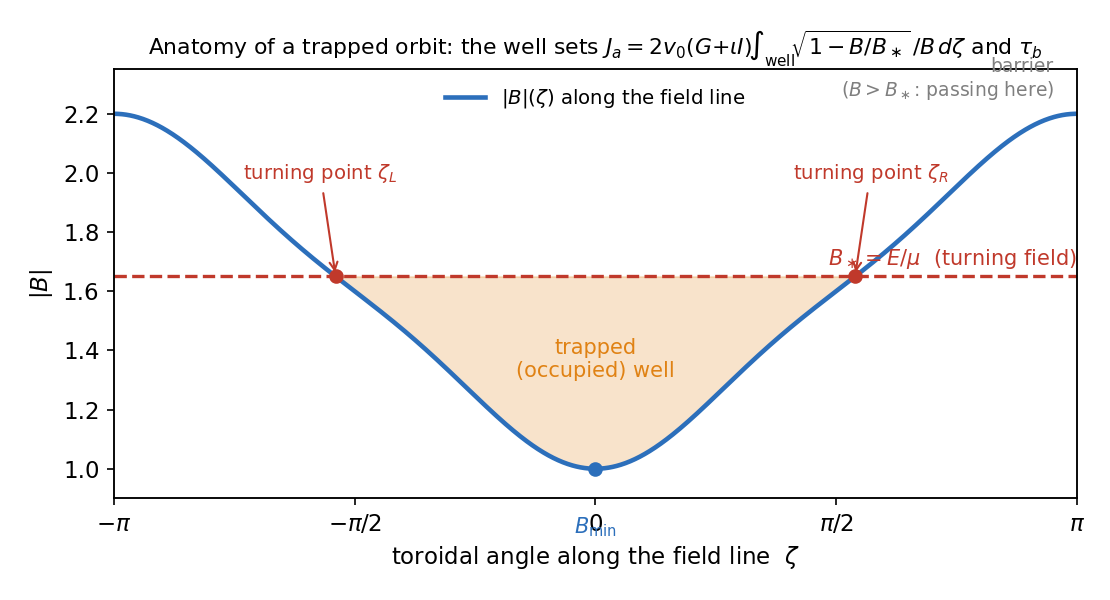
\includegraphics[width=0.86\linewidth]{figures/anatomy_of_a_well.png}
  \caption{\textbf{Anatomy of a trapped orbit.} $|B|$ along a field line. The particle with
  turning field $\Bstar=E/\mu$ is trapped in the shaded well between the turning points
  $\zeta_L,\zeta_R$ (where $B=\Bstar$). The well fixes the bounce integrals $J_a$ and $\tau_b$.
  The turning points and well shown are computed by the actual engine
  (\code{find\_wells}/\code{integrate\_well}).}
  \label{fig:well}
\end{figure}

% ============================================================================
\section{Definition of \GW}

\subsection{Bounce integrals}
For the occupied well of a trapped alpha ($v_0=\sqrt{2E/m_\alpha}$ its speed, Boozer arc length
$d\ell=|G+\ii I|/B\,d\zeta$), the physical full-bounce second adiabatic invariant and bounce time
are
\begin{align}
  J_a(s,\alpha)   &= 2\,v_0\,(G+\ii I)\!\int_{\rm well}\!\frac{\sqrt{1-B/\Bstar}}{B}\,d\zeta
                     \qquad [\mathrm{m^2/s}], \label{eq:J}\\[0.3em]
  \tau_b(s,\alpha)&= \frac{2}{v_0}\,(G+\ii I)\!\int_{\rm well}\!\frac{1}{B\,\sqrt{1-B/\Bstar}}\,d\zeta
                     \qquad [\mathrm{s}]. \label{eq:tau}
\end{align}
$J$ (equivalently $J_\parallel=\oint v_\parallel\,d\ell$) is the \emph{second adiabatic
invariant}, conserved when the field varies slowly over a bounce---the whole method rests on
$J$ being an invariant of the drift. $\tau_b$ is the bounce period; the $1/\sqrt{1-B/\Bstar}$
factor diverges \emph{integrably} at the turning points and is integrated analytically per grid
cell (\S\ref{sec:num}).

\subsection{The bounce-centre drift (Whitham characteristic)}
The bounce centre drifts along level sets of $J$ at fixed $(E,\mu)$. The signed,
time-parametrized characteristic is
\begin{equation}
  \boxed{\;\dot s = +\frac{\kappa}{\tau_b}\,\frac{\partial J}{\partial\alpha},\qquad
          \dot\alpha = -\frac{\kappa}{\tau_b}\,\frac{\partial J}{\partial s},\qquad
          \kappa = \mathrm{sign_{conv}}\,\frac{m_\alpha}{Z_\alpha e\,\Psi_{\rm LCFS}}\;}
  \label{eq:char}
\end{equation}
$\kappa$ fixes the absolute drift rate: $m_\alpha, Z_\alpha e$ are the alpha mass and charge and
$\Psi_{\rm LCFS}=|\psi_0|=\Phi_{\rm edge}/2\pi$ is the edge toroidal flux over $2\pi$ (the Boozer
canonical-momentum normalization). \textbf{This is taken from the field's definition, not
fitted}; $\mathrm{sign_{conv}}=+1$ was fixed once by the Landreman gate (\S\ref{sec:val}) and
never changed.

Why $\partial J/\partial\alpha$ is radial drift: Eq.~\eqref{eq:char} is the bounce-averaged
grad-$B$/curvature drift in action--angle form, exactly analogous to $\dot x=\partial H/\partial
p$. A field in which $J$ does \emph{not} depend on $\alpha$ (an \textbf{omnigeneous} / perfectly
quasisymmetric field) has $\dot s=0$: no radial drift, perfect trapped confinement. \GW\
therefore measures the residual $\alpha$-dependence of $J$ that quasisymmetry breaking
introduces.

\subsection{Per-marker reach and the configuration objective}
Integrating Eq.~\eqref{eq:char} for each launched particle (``marker'') $i$ to endpoint $t_\ast$,
\begin{align}
  R_{W,i}(t_\ast) &= \mathrm{clip}\!\left[\frac{\max_{0\le t\le t_\ast}s_i(t)-s_{0,i}}{1-s_{0,i}},\,0,\,1\right],
      \label{eq:RW}\\[0.3em]
  \GW(t_\ast)     &= \frac{\sum_i w_i\,R_{W,i}}{\sum_i w_i}\quad\text{(primary objective)},\qquad
  L_W(t_\ast) = \frac{\sum_i w_i\,\mathbf{1}[s_{\max,i}\ge 1]}{\sum_i w_i}\ \text{(diagnostic)}.
      \label{eq:GW}
\end{align}
$R_W$ is the normalized radial reach of one marker ($0$ = stays at launch surface, $1$ = reaches
the edge). \GW\ is the source-averaged reach over all markers, with $w_i$ the source quadrature
weight of an isotropic, volume-uniform source on $s_0$---a single scalar per configuration.
$L_W$ (weight that hit the edge) is kept only as a diagnostic, because a binary
reached/didn't-reach throws away the graded reach that makes \GW\ robust. $t_\ast$ is the only
geometry-dependent knob: the physical time over which one asks ``how far can it drift''---e.g.\ a
slowing-down time ($0.2$~s) or a prompt-loss window ($10$~ms). \GW\ is a \emph{prompt-excursion}
metric (see \S\ref{sec:scope}).

\begin{figure}[htbp]
  \centering
  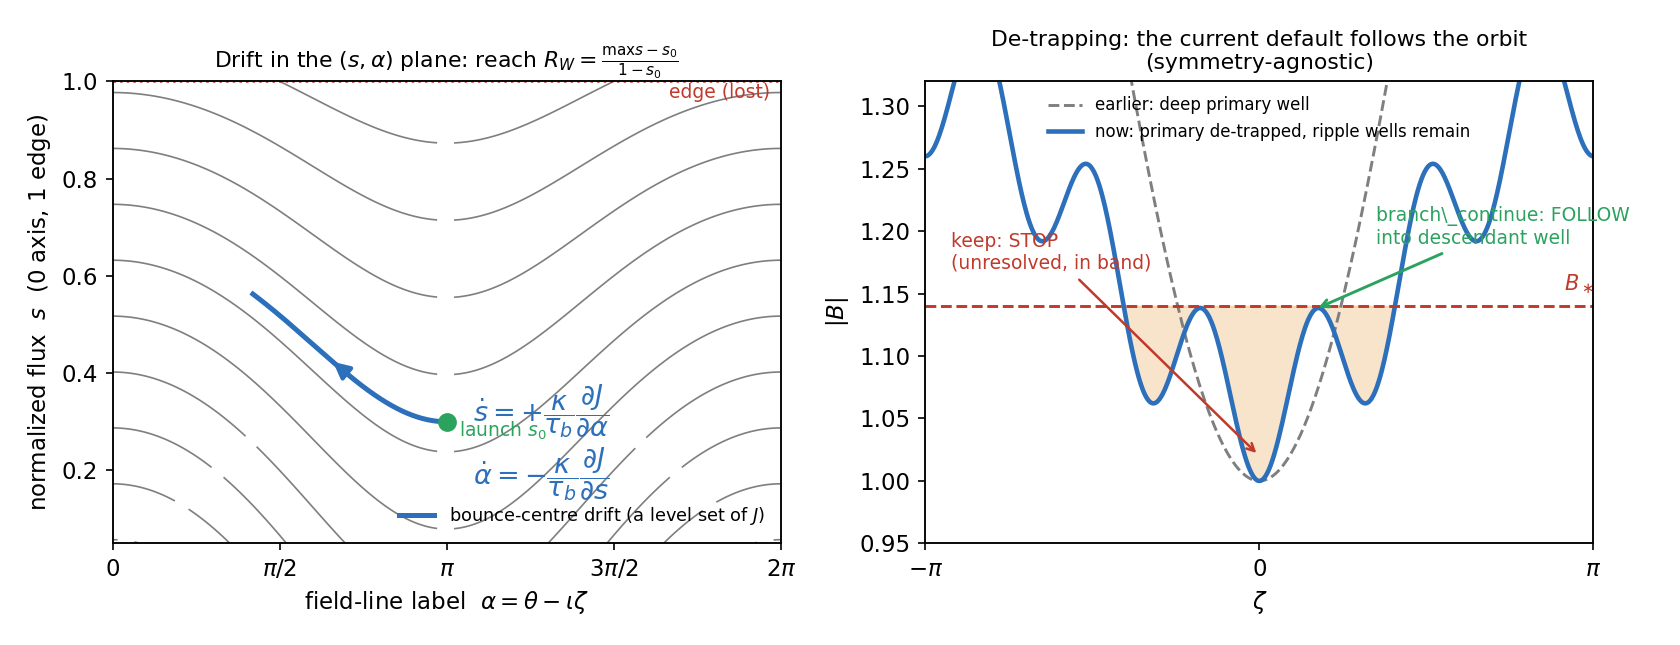
\includegraphics[width=\linewidth]{figures/drift_and_detrapping.png}
  \caption{\textbf{Left:} the bounce centre drifts along a level set of $J$ in the $(s,\alpha)$
  plane; the radial reach $R_W$ is its furthest excursion toward the edge, normalized by
  $1-s_0$. \textbf{Right:} a de-trapping event---the occupied (primary) well has become too
  shallow to hold the particle while ripple/secondary wells remain. The published ``keep'' metric
  \emph{stops} (marks the marker unresolved, in the band); the current default
  \code{branch\_continue} \emph{follows} the orbit into the descendant well and lets its own
  drift decide the fate (\S\ref{sec:detrap}).}
  \label{fig:drift}
\end{figure}

% ============================================================================
\section{De-trapping and the branch-continued Whitham}
\label{sec:detrap}

The adiabatic picture assumes the particle stays in \emph{one} well for the whole time. Real
trapped orbits can \textbf{de-trap}: as the bounce centre drifts, its occupied well can become
too shallow and vanish ($\Bstar$ rises above the local $B_{\min}$) or split. What happens next
decides confinement and is the crux of the current version.

In a \textbf{quasisymmetric stellarator} de-trapping usually means the orbit becomes passing or
re-traps in an equivalent well and stays confined. In a \textbf{tokamak with toroidal-field
ripple} (or a symmetry-broken region) de-trapping can drop the particle into a \textbf{ripple
well}, whose vertical grad-$B$ drift does \emph{not} bounce-average to zero, so the particle
walks radially out and is lost. A naive metric that simply stops at the de-trapping event gets
this backwards and produces spurious \emph{non-monotonic dips} in \GW\ vs.\ ripple.

Three treatments are available on \code{GWParams}:
\begin{enumerate}[nosep,leftmargin=1.4em]
  \item \textbf{\code{branch\_continue=True} --- default, recommended.} The symmetry-agnostic
        branch-continued Whitham. At a de-trapping event the code does not guess---it
        \emph{follows} the orbit into the descendant (ripple/secondary) well (found by
        maximum-interval overlap, stepped with clipped Euler because RK4 re-blows-up the fragile
        ripple-well finite differences) and lets that well's own bounce-averaged radial drift
        decide lost vs.\ confined. With no descendant well the orbit is \code{DETRAP\_PASSING}
        (de-trapped to passing $\to$ confined). Using no symmetry assumption, it works uniformly
        on quasi-axisymmetric (QA), quasi-helical (QH), axisymmetric, \emph{and} mixed-symmetry
        fields. \code{branch\_continue=False} recovers the exact original ``keep'' metric
        bit-for-bit.
  \item \textbf{\code{detrap\_fate=True} --- superseded (kept for reference).} The older
        $\delta_{\rm QS}$ classifier calls a de-trapped orbit lost if the local
        quasisymmetry-breaking $\delta_{\rm QS}$ (the $|B|$ variation along the QS-invariant
        helix) exceeds a threshold $\eta_{\rm ripple}$. It needs a \emph{dominant} helicity, so
        it is meaningless on mixed symmetry and over-corrected some QA cases; replaced by
        \code{branch\_continue}.
  \item \textbf{\code{branch\_continue=False} (keep).} Stops at the de-trapping event and keeps
        the reach so far. Under-counts loss where de-trapping leads to ripple-trapping, producing
        the non-monotonic dips.
\end{enumerate}

\textbf{Validated behaviour.} \code{branch\_continue} is byte-identical to the published keep
metric on the good QA/QH/mixed legacy sets --- it is \emph{inert} where orbits stay adiabatically
confined. The direct same-engine comparison (identical markers, \code{branch\_continue} the only
difference) gives rank agreement $\mathbf{0.9999}$--$\mathbf{1.0000}$ on all three legacy datasets:
it fires in proportion to de-trapping (4/250 configs on Alex, both QA configs on Paul, 2645
continuation hops on the mixed-symmetry Landreman cfg4) and still does not change the ordering.

On a \emph{rippled} field, where de-trapping drives the transport, a branch-aware treatment is what
removes the spurious dip; Fig.~\ref{fig:qh} shows this qualitatively on the QH ripple scan. The
quantified statement supported by a frozen artifact is the de-trapping \emph{fate} treatment on the
rippled tokamak: Spearman-vs-loss rises from $0.05$ (keep) to $\mathbf{0.93}$ at $n{=}2$, and from
$0.58$ to $\mathbf{0.96}$ at $n{=}3$ (\code{gamma\_w\_n\{2,3\}\_fate.csv}, $\eta=0.02$; robust over
$\eta\in[0.01,0.03]$). Option~2 is superseded as a \emph{general} default because $\delta_{\mathrm{QS}}$
needs a dominant helicity --- but this is the one geometry where it is well posed: for a tokamak/QA
($N{=}0$) the QS-invariant direction \emph{is} the toroidal direction, so $\delta_{\mathrm{QS}}$
reduces exactly to the raw ripple. A branch-continued equivalent of those two numbers has \emph{not} been
re-frozen on the current engine and is deliberately not quoted here. See \S\ref{sec:val}.

% ============================================================================
\section{Outputs, band, and regime flags}
\label{sec:outputs}

\code{gamma\_w\_for\_boozmn(...)} returns a dictionary and (verbose) prints, e.g.
\begin{Verbatim}[fontsize=\small,frame=single,rulecolor=\color{gray},samepage=true]
  nfp=4 Psi_LCFS=6.6628  N=128 t*=0.2s s0=0.3  branch_continue=True fate=False
  Gamma_W = 0.00516   L_W = 0.0000   [adiabatic-resolved]
  band [low,high] = [0.00516, 0.00516]
  passing_frac = 0.648  unresolved = 0.000  branch_event = 0.000
\end{Verbatim}

\begin{center}\small
\begin{tabular}{@{}p{0.28\linewidth}p{0.66\linewidth}@{}}
\toprule
field & meaning \\
\midrule
\code{Gamma\_W} & the headline reach (the ``keep'' aggregation of resolved reaches). \\
\code{L\_W} & loss-fraction proxy (weight with $s_{\max}\ge1$); diagnostic only. \\
\code{Gamma\_W\_low} / \code{\_high} & the \textbf{uncertainty band}: score every
   \emph{unresolved} marker's reach as $0$ (low, pessimistic) or $1$ (high, optimistic). The
   truth for a de-trapped orbit lies in the band; when de-trapping $\to$ ripple-trapping $\to$
   loss the \emph{high} edge is correct. Report the band, not just the point. \\
\code{regime} & a plain-language trust flag (below). \\
\code{passing\_frac} & source weight passing at birth ($R_W=0$); if $>0.85$ the trapped-only
   \GW\ is blind to most of the source. \\
\code{branch\_event\_w\_frac} & source weight that hit an unresolved de-trapping/branch event. \\
\code{unresolved\_w\_frac} & source weight whose characteristic could not be cleanly resolved
   (any event/guard status). \emph{Never} silently converted to a loss. \\
\code{n\_cont\_rescues} & (per marker) total branch-continuation rescues, including those fired
   inside an RK4 substage; $\ge$ \code{n\_branch}. See \S\ref{sec:integrity}. \\
\bottomrule
\end{tabular}
\end{center}

\textbf{Regime flag} (the ``read-me'' for the number):
\begin{itemize}[nosep]
  \item \code{adiabatic-resolved} ($\mathrm{bevent}\le0.20$, $\mathrm{passing}\le0.85$) --- \GW\
        (keep) is trustworthy; the band is tight.
  \item \code{de-trapping-dominated} ($\mathrm{bevent}>0.20$) --- many orbits de-trap; the point
        estimate is under-resolved $\to$ read the $[\mathrm{low,high}]$ band and prefer
        \code{branch\_continue}.
  \item \code{passing-dominated} ($\mathrm{passing}>0.85$) --- most of the source is passing; a
        trapped-only reach metric is blind here.
\end{itemize}

\textbf{Per-marker status codes.} \code{ok\_confined}, \code{ok\_lost} (reached edge),
\code{detrap\_passing} (branch-continued to passing $\to$ confined), \code{ripple\_lost}
($\delta_{\rm QS}$ fate: ripple-trapped $\to$ lost), \code{passing} (passing at birth), and the
\emph{unresolved} set \code{branch\_event\_unresolved}, \code{tau\_guard\_unresolved},
\code{fd\_branch\_mismatch\_unresolved}, \code{step\_cap\_unresolved}, \code{field\_eval\_failed},
\code{no\_launch}. Only \code{ok\_lost}/\code{ripple\_lost} contribute to $L_W$; \emph{all}
statuses keep their verified $s_{\max}\to R_W$. A numerical failure is never mapped to a physical
outcome (\S\ref{sec:integrity}).

% ============================================================================
\section{Numerical method (why it is trustworthy)}
\label{sec:num}

\begin{itemize}[nosep]
  \item \textbf{Turning-point-aware bounce quadrature (the verifiable core).} The integrands in
        Eqs.~\eqref{eq:J}--\eqref{eq:tau} carry an integrable $1/\sqrt{1-B/\Bstar}$ singularity at
        the turning points. Rather than a numerical floor, the code takes $g\equiv1-B/\Bstar$
        \emph{linear across each grid cell} and integrates $\sqrt{g}$ and $1/\sqrt{g}$
        \emph{analytically} per cell (prefactor cell-averaged). Validated against
        \code{scipy.quad} to $\sim10^{-5}$ on parabolic and cosine model wells across depths
        $q_\ast=0.05$--$0.8$ (\code{python Gamma\_W\_final.py -{}-selftest}).
  \item \textbf{Predictive single-shot ODE stepping.} The step is set so both
        $|\Delta s|<\code{ds\_step\_max}$ ($0.02$) and $|\Delta\alpha|<\code{dalpha\_step\_max}$
        ($0.03$) in one shot---\emph{no} adaptive retries in the singular de-trapping regions
        (retries re-trigger the blow-up). If the required step falls below a floor, the marker is
        flagged \code{step\_cap\_unresolved} rather than crawling.
  \item \textbf{Branch-event guard ladder.} Before $\dot s$ can blow up near a vanishing well,
        guards fire: descendant-well overlap/continuity; well too shallow
        ($\Bstar-B_{\min}<\eta_B(B_{\max}-B_{\min})$, $\eta_B=10^{-4}$); trapped width
        $<4\,\Delta\zeta_{\rm grid}$; $\tau_b$ non-finite or $<\eta_\tau\cdot\mathrm{median}$
        ($\eta_\tau=10^{-3}$); finite-difference branch mismatch. Each event stops and keeps the
        verified reach; unresolved fractions are reported, never silently turned into losses.
  \item \textbf{Closed-orbit / stall early exits.} Bounded (confined) orbits are detected by
        first-peak / no-radial-progress tests so they do not crawl for thousands of steps. This
        is a prompt-reach approximation, justified because a monotone escaper cannot be truncated
        and a librating orbit's first excursion bounds its reach (see the early-stop analysis in
        the review record).
\end{itemize}

% ============================================================================
\section{The Nemov \Gc\ sibling}
\label{sec:gammac}

\code{gamma\_c.py} computes Nemov's contour-inclination proxy \Gc\ as a \emph{read-only
by-product} of the same pipeline. Per trapped marker at its launch,
\begin{equation}
  \gamma_c = \frac{2}{\pi}\,\mathrm{atan2}\!\big(|\partial J/\partial\alpha|,\,
             |\partial J/\partial s|\big)\ \in[0,1],
\end{equation}
with the derivatives taken from \GW's own \code{\_rhs} at $t=0$ (no ODE, no branch continuation),
so they are bit-identical to the \GW\ drift by construction---the common $\tau_b/\kappa$ factor
cancels inside $\mathrm{atan2}$. It aggregates as the weighted mean of $\gamma_c^2$ over trapped
markers ($\Gamma_{c,\mathrm{trapped}}$) or over the full source ($\Gamma_{c,\mathrm{source}}$). \Gc\ is a launch-point
(one-shot) statistic by construction; the comparison against the path-integrated \GW\ is the
scientific point. On Alex-250, $\Gamma_{c,\mathrm{trapped}}$ Spearman-vs-loss $=0.446$, below \GW\ ($0.656$)
and QS ($0.736$)---consistent with \GW's radial-reach integration adding skill over the
launch-point angle.

% ============================================================================
\section{Using the code}

\subsection{Command line}
\begin{Verbatim}[fontsize=\small,frame=single,rulecolor=\color{gray}]
# a process with firm3d (NOT simsopt in the same process -- a pybind11 clash):
source /opt/miniconda3/etc/profile.d/conda.sh && conda activate simsopt

python Gamma_W_final.py --selftest                    # quadrature self-test (no firm3d)
python Gamma_W_final.py --boozmn FILE.nc               # score one equilibrium (branch_continue ON)
python Gamma_W_final.py --boozmn FILE.nc --keep        # disable branch_continue (exact keep metric)
python Gamma_W_final.py --boozmn FILE.nc --N 256 --t-star 0.2 --s0 0.3 --seed 7
\end{Verbatim}
\code{FILE.nc} is a VMEC \code{wout} \emph{or} a \code{booz\_xform} \code{boozmn} file (built with
\code{flux=True}). \code{-{}-keep} recovers the published pre-branch\_continue numbers exactly.

\subsection{Python}
\begin{Verbatim}[fontsize=\small,frame=single,rulecolor=\color{gray}]
from Gamma_W_final import gamma_w_for_boozmn

agg = gamma_w_for_boozmn(
        "wout.nc",
        N=128,          # isotropic, volume-uniform markers on s0
        t_star=0.2,     # endpoint [s]
        s0=0.3,         # launch surface
        seed=7,
        branch_continue=True)   # DEFAULT symmetry-agnostic de-trapping treatment
# agg['Gamma_W'], agg['Gamma_W_low'/'_high'], agg['regime'],
# agg['branch_event_w_frac'], agg['passing_frac'], agg['L_W'], ...
\end{Verbatim}

\textbf{Key objects.} \code{FieldBundle} wraps a firm3d \code{InterpolatedBoozerField} (exposes
\code{modB}, \code{profiles}$\to(G,I,\ii)$, \code{Psi\_LCFS}, \code{nfp}, \code{helicity}, and an
$s$-clamp guarding an out-of-domain firm3d segfault). \code{GWParams} is the parameter dataclass
(quadrature resolution, finite-difference steps, ODE stepping, guard thresholds, and the
de-trapping switches). \code{make\_surface\_markers} is the isotropic source;
\code{integrate\_characteristic} is the signed Whitham ODE with the guard ladder;
\code{aggregate} turns per-marker rows into \GW, the band, the regime flag, and the fractions.

\textbf{Environment.} firm3d must be imported in a process that does \emph{not} import
\code{simsopt} (pybind11 clash); VMEC (to \emph{make} equilibria) uses simsopt, so generation and
scoring run in separate processes.

% ============================================================================
\section{Validation history and the converged verdict}
\label{sec:val}

\begin{center}\small
\begin{tabular}{@{}p{0.24\linewidth}p{0.30\linewidth}p{0.40\linewidth}@{}}
\toprule
dataset & what & result \\
\midrule
Quadrature self-test & $J,\tau_b$ vs.\ \code{scipy.quad} & rel.\ err $\le4\times10^{-5}$ \\
Landreman gate (mixed nfp=4, vs.\ FIRM3D) & normalization + mechanism &
   \GW: cfg5\_prompt $\mathbf{0.701}$ $>$ cfg5\_confined $0.394$ $>$ cfg4\_control $\mathbf{0.076}$;
   $\dot s_W/$FIRM3D $\mathcal{O}(1)$ from definitions \\
Paul (5 reactor configs) & rank loss & mechanism right; per-config reach under-predicts trapped
   QA banana loss (boundary result) \\
Alex (250 QH perturbations) & rank loss & amplitude trend near-perfect ($\sigma$-bin-median
   $0.985$); Spearman $0.656<$ QS $0.736$ \\
Rippled tokamak ($n{=}2,3$) & resolve the de-trapping dip & keep Spearman $0.05\to$ de-trapping
   fate $\mathbf{0.93}$ ($n{=}2$); $0.58\to\mathbf{0.96}$ ($n{=}3$), $\eta=0.02$; base axisymmetric
   case stays exactly $0$ \\
keep vs.\ \code{branch\_continue} & do rankings change? & rank agreement
   $\mathbf{0.9999}$--$\mathbf{1.0000}$ on Alex-250 / Paul / Landreman --- active but
   rank-preserving \\
QH toroidal ripple & behaviour on QH + ripple & Fig.~\ref{fig:qh} \\
\bottomrule
\end{tabular}
\end{center}

\begin{figure}[htbp]
  \centering
  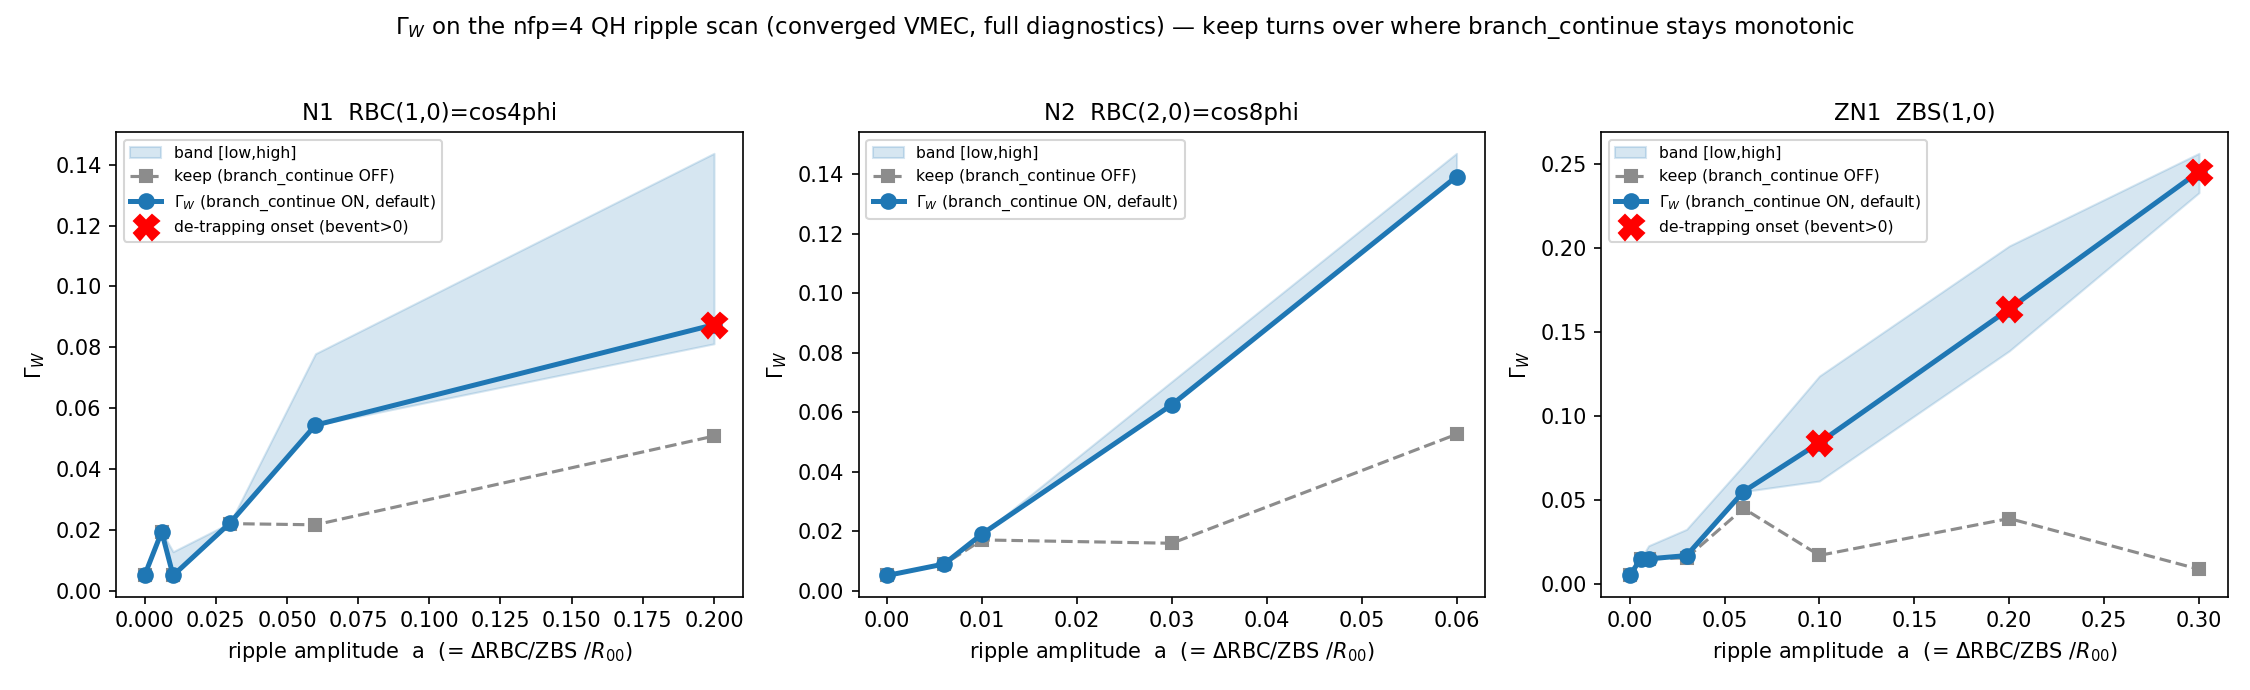
\includegraphics[width=0.92\linewidth]{figures/qh_ripple_diagnostic.png}
  \caption{\textbf{QH toroidal-ripple test.} Where de-trapping onsets, the raw \emph{keep} metric
  turns over non-monotonically (the ``dip'') while the branch-continued \GW\ stays monotonic in
  ripple amplitude, with the $[\mathrm{low,high}]$ band bracketing it. The dip is the
  \code{branch\_continue=OFF} signature; the band + regime flag are the recommended read for a
  ripple scan.}
  \label{fig:qh}
\end{figure}

\textbf{Converged verdict (unchanged).} \GW's leading-order \emph{adiabatic reach} captures the
loss \emph{mechanism} (Landreman gate) and the \emph{amplitude scaling} (Alex $\sigma$-bin-median
$0.985$), but is \emph{not} a drop-in quantitative replacement for the quasisymmetry error QS: on
the full Alex-250 it trails QS ($0.656$ vs.\ $0.736$), and on Paul it under-predicts trapped-channel
QA banana loss. The missing ingredient is the finite-orbit-width / non-adiabatic drift that a
field-only proxy omits by construction. \GW\ is best used as a \textbf{mechanism / amplitude /
ripple diagnostic}, not a predictive surrogate for QS. No fitted multipliers or dataset-specific
coefficients enter: the only geometry-dependent knob is $t_\ast$.

% ============================================================================
\section{Code integrity, provenance, and tests}
\label{sec:integrity}

The canonical engine is the single file \code{Gamma\_W\_final.py}. Its identity is pinned by md5;
the lineage of the current release is
\begin{center}\small
\code{9de057ad} $\to$ \code{5952f45f} $\to$ \code{575187cf} $\to$ \code{b58272e4}\quad(the file shipped here).
\end{center}
Two July-13 patches produced this lineage; both are score-preserving on the published ``keep''
metric and are covered by regression tests.
\begin{itemize}[nosep]
  \item \textbf{P1 / status propagation (\code{9de057ad}$\to$\code{5952f45f}).} Previously a
        \emph{numerical} finite-difference mismatch (a valid well but a failed drift stencil) could
        fall through to the ODE substepper and, under \code{branch\_continue}, be mis-scored
        \code{DETRAP\_PASSING} (physically confined, outside the band). Now any non-``ok'' status
        stops the marker, preserves $s_{\max}$, and is flagged \emph{unresolved} with its
        originating status; only a genuinely empty descendant well yields \code{DETRAP\_PASSING}.
        A numerical failure is never mapped to a physical outcome. keep-mode \GW\ is numerically
        unchanged.
  \item \textbf{\code{n\_cont\_rescues} counter (\code{5952f45f}$\to$\code{575187cf}).}
        Diagnostic-only. The internal \code{n\_branch} counter misses continuation rescues that
        fire inside an RK4 substage; \code{n\_cont\_rescues} is a persistent tally of \emph{every}
        rescue and satisfies $\code{n\_cont\_rescues}\ge\code{n\_branch}$. It is never read by
        control flow, so all scores (keep and branch-continue) are byte-identical.
\end{itemize}

\textbf{Test suite.} A \code{pytest} suite (shipped in \code{tests/}) locks the engine: a fast
pure-numpy \code{unit} tier (turning-point quadrature vs.\ \code{scipy.quad}, well detection, the
$\Bstar/\kappa$ normalizations, occupied-well action, the aggregation band/regime logic, the
$\gamma_c$ angle, and the control-ladder decisions via mocked field evaluations---including the
keep-vs-branch-continue dispatch and the two patches above), plus a firm3d-dependent
\code{regression}/\code{slow} tier that scores a small shipped QA \code{boozmn} against frozen
values. Run \code{pytest -m unit} for the $<1$~s firm3d-free lane.

\textbf{Ripple-scan generator (\code{scripts/create\_scan.py}).} The tool that adds boundary
ripple for the ripple-scan gate had two boundary-corruption bugs (an exponent-strip parse bug and
a \code{reset()} list-aliasing bug that accumulated ripple across scan iterations); both are fixed
and locked by \code{tests/test\_create\_scan.py} (a zero-perturbation-identity + non-accumulation
regression test). Scan \emph{equilibria} must be regenerated with the fixed generator before any
ripple-scan number is cited.

% ============================================================================
\section{Scope and limitations}
\label{sec:scope}

\begin{itemize}[nosep]
  \item \GW\ is a \textbf{prompt-excursion} metric. Full-interval integration to a slowing-down
        time ($t_\ast=0.2$~s) is both intractable ($\sim10^4$--$10^5$ steps/marker) and outside
        the validity of a collisionless adiabatic model over a slowing-down time; the metric is
        therefore defined and used as a prompt radial-reach quantity.
  \item It is \textbf{field-only and adiabatic}: it omits the finite-orbit-width / non-adiabatic
        drift, so it captures loss \emph{mechanism} and \emph{amplitude scaling} but is not a
        quantitative surrogate for QS.
  \item It is a \textbf{trapped-population} metric: passing fraction is reported, and a
        \code{passing-dominated} configuration ($>85\%$ passing) is flagged as one where a
        trapped-only reach is blind.
  \item On a ripple scan the source-averaged reach is intrinsically \emph{bumpy} (a threshold
        quantity: markers cross the edge non-monotonically), independent of de-trapping---fit a
        trend and read the band, do not over-read individual points.
\end{itemize}

% ============================================================================
\section{Package contents and reproduction}

\begin{Verbatim}[fontsize=\small,frame=single,rulecolor=\color{gray}]
Gamma_W_standalone/
  Gamma_W_doc.{tex,pdf,md}         <- this document (three formats)
  Gamma_W_final.py                 <- canonical engine (md5 b58272e4)
  gamma_c.py                       <- Nemov Gamma_c sibling (read-only by-product)
  README.md                        <- quickstart + manifest
  scripts/
    create_scan.py                 <- ripple-scan boundary generator (P5-fixed)
    make_doc_figures.py            <- regenerates figures/anatomy + drift_and_detrapping
  figures/
    anatomy_of_a_well.png          <- Fig 1 (engine-generated)
    drift_and_detrapping.png       <- Fig 2 (engine-generated)
    qh_ripple_diagnostic.png       <- Fig 3 (QH-ripple validation)
  pyproject.toml                   <- pytest markers (unit/regression/slow)
  tests/
    conftest.py test_core.py test_dynamics.py test_gamma_c.py test_regression.py
                                   <- pytest suite (unit + regression) + test_files/ QA boozmn
    test_create_scan.py            <- ripple-generator regression test
\end{Verbatim}

\textbf{Reproduce a self-test and a single score} (run from the package root):
\begin{Verbatim}[fontsize=\small,frame=single,rulecolor=\color{gray}]
conda activate simsopt
python Gamma_W_final.py --selftest
python Gamma_W_final.py --boozmn <wout_or_boozmn>.nc --N 128 --t-star 0.2 --s0 0.3
pytest -m unit          # <1 s, no firm3d (43 tests)
\end{Verbatim}

\vfill
\begin{center}\small\itshape
The only geometry-dependent knob is the physical endpoint $t_\ast$.\\
\code{branch\_continue=True} is the default; \code{-{}-keep} recovers the published keep-metric exactly.
\end{center}

\end{document}
